\title{Understanding the relative contributions of individual protonation states in PIP$_3$ and PIP$_2$ lipid towards free energy of binding of AKT1 protein with membrane}
\author{Krishnakanth B}
\date{\today}

\documentclass[12pt]{article}
\usepackage[left=10mm, right=10mm, top=5mm, bottom=5mm]{geometry}
\usepackage{hyperref}
\usepackage{float}
\usepackage{graphicx}
\usepackage{amsmath}
\begin{document}
\maketitle



\paragraph{}
The concentrations of individual states of PIP$_3$ are represented using $[345]$, $[34'5]$, $[345']$, $[3'45]$,
$[34'5']$, $[3'45']$, $[3'4'5]$ and $[3'4'5']$. Similarly, the concentrations of individual protonation states of 
PIP$_2$ are represented using $[45]$,$[4'5]$,$[45']$ and $[4'5']$.

We adopted the equations from reference\cite{graber2018effect} and re-wrote them 
to get the functional forms of fraction of individual protonation states of PIP$_3$ and PIP$_2$.
Using equations set \ref{eq1}, \ref{eq3} in \ref{eq2} and \ref{eq4} respectively, we could reproduce the fraction of each protonation state 
of PIP$_3$ and PIP$_2$ respectively as function of pH. We further quantified the uncertainity of each of these fractions using the
error on the $pK_{a}$s as reported in \cite{graber2018effect}.


\subsection*{PIP$_3$}
\begin{equation} \label{eq1}
\begin{split}
[3'45] & = [345] 10^{pH-pK_{a1}} \\
[34'5] & = [345] 10^{pH-pK_{a2}} \\
[345'] & = [345] 10^{pH-pK_{a3}} \\
[3'4'5] & = [345] (10^{2pH-pK_{a1}-pK_{a7}} + 10^{2pH-pK_{a2}-pK_{a9}} ) \\
[3'45'] & = [345] (10^{2pH-pK_{a1}-pK_{a8}} + 10^{2pH-pK_{a3}-pK_{a11}} ) \\
[34'5'] & = [345] (10^{2pH-pK_{a2}-pK_{a10}} + 10^{2pH-pK_{a3}-pK_{a12}} ) \\
[3'4'5'] & = [345] \huge(10^{3pH-pK_{a1}-pK_{a7}-pK_{a16}} + 10^{3pH-pK_{a2}-pK_{a9}-pK_{a16}} \\
& + 10^{3pH-pK_{a1}-pK_{a8}-pK_{a17}} + 10^{3pH-pK_{a3}-pK_{a11}-pK_{a17}}  \\
& + 10^{3pH-pK_{a2}-pK_{a10}-pK_{a18}} + 10^{3pH-pK_{a3}-pK_{a12}-pK_{a18}} \huge)
\end{split}
\end{equation}


\begin{equation} \label{eq2}
\begin{split}
f_{3'45} & = \frac{[3'45]}{[345]+[3'45]+[34'5]+[345']+[3'4'5]+[3'45']+[34'5']+[3'4'5']} \\
f_{34'5} & = \frac{[34'5]}{[345]+[3'45]+[34'5]+[345']+[3'4'5]+[3'45']+[34'5']+[3'4'5']} \\
f_{345'} & = \frac{[345']}{[345]+[3'45]+[34'5]+[345']+[3'4'5]+[3'45']+[34'5']+[3'4'5']} \\
f_{3'4'5} & = \frac{[3'4'5]}{[345]+[3'45]+[34'5]+[345']+[3'4'5]+[3'45']+[34'5']+[3'4'5']} \\
f_{3'45'} & = \frac{[3'45']}{[345]+[3'45]+[34'5]+[345']+[3'4'5]+[3'45']+[34'5']+[3'4'5']} \\
f_{34'5'} & = \frac{[34'5']}{[345]+[3'45]+[34'5]+[345']+[3'4'5]+[3'45']+[34'5']+[3'4'5']} \\
f_{3'4'5'} &  = \frac{[3'4'5']}{[345]+[3'45]+[34'5]+[345']+[3'4'5]+[3'45']+[34'5']+[3'4'5']} \\
f_{345} & = 1-(f_{3'45}+f_{34'5}+f_{345'}+f_{3'4'5}+f_{3'45'}+f_{34'5'}+f_{3'4'5'})
\end{split}
\end{equation}

\subsection*{PIP$_2$}

\begin{equation} \label{eq3}
\begin{split}
[4'5] & = [45] 10^{pH-pK_{a1}}  \\
[45'] & = [45] 10^{pH-pK_{a2}} \\
[4'5'] & = [4'5] 10^{pH-pK_{a4}} + [45'] 10^{pH-pK_{a5}} \\
& = [45] (10^{2pH-pK_{a1}-pK_{a4}}  + 10^{2pH-pK_{a2}-pK_{a5}}) \\
\end{split}
\end{equation}


\begin{equation} \label{eq4}
\begin{split}
f_{4'5} & = \frac{[4'5]}{[45]+[4'5]+[45']+[4'5']} \\
f_{45'} & = \frac{[45']}{[45]+[4'5]+[45']+[4'5']} \\
f_{4'5'} &  = \frac{[4'5']}{[45]+[4'5]+[45']+[4'5']} \\
f_{45} & = 1-(f_{4'5}+f_{45'}+f_{4'5'})
\end{split}
\end{equation}

\begin{figure}[H] 
\begin{center}
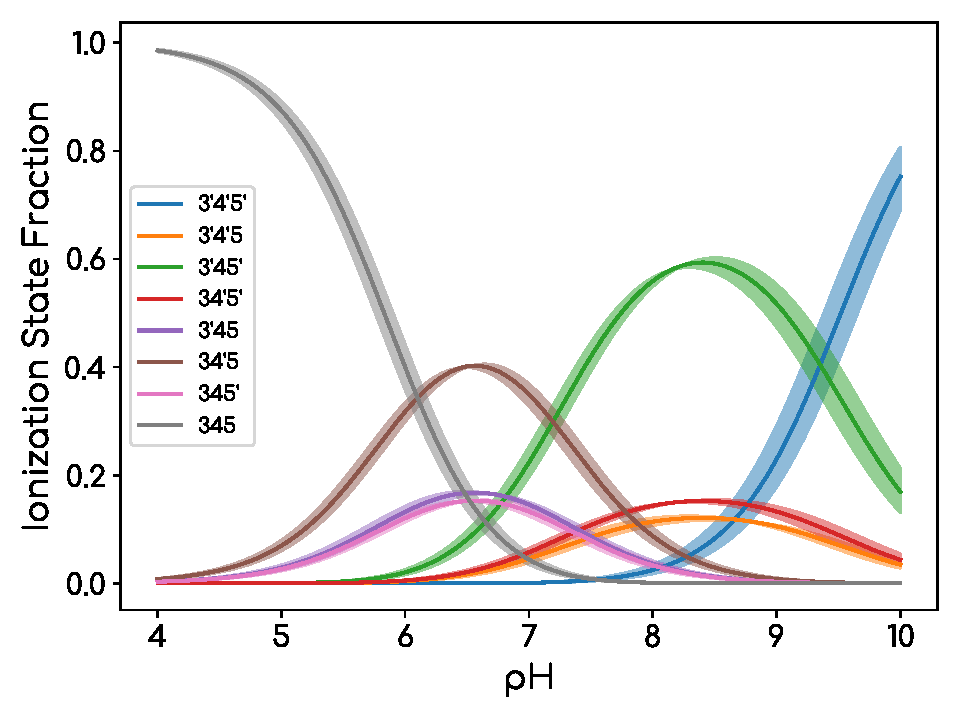
\includegraphics[width=0.45\linewidth]{figs/pip3_ionization_fractions.pdf}
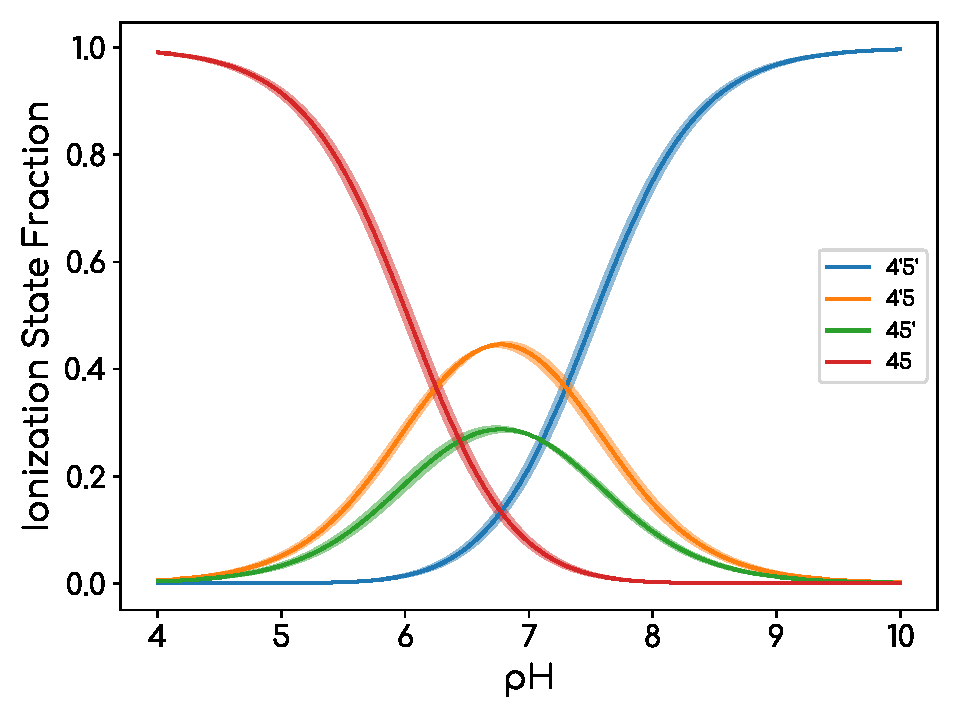
\includegraphics[width=0.45\linewidth]{figs/pip2_ionization_fractions.pdf}
\caption{Fraction of each protonation state of PIP$_3$ (left) and PIP$_2$ (right) as a function of pH}
\label{figure1}
\end{center}
\end{figure}


These analytical forms were used along with the free energy of binding obtained from umbrella sampling simulations to evaluate 
the free energy of binding as a function of pH $(\Delta G^{sim}_{binding}(pH))$ using eqn.\ref{eqn_G}  (shown in figure \ref{figure2}). The uncertainity $(\Delta G_{error})$ on these curves 
were evaluated using primitive error propagation relations (eqn.\ref{error_eqn}), accounting for (i) Uncertainity on fraction of each protonation 
state$(f_{i,error}(pH))$ using error evaluated on $pK_a$s of the above model\cite{graber2018effect}. (ii) Uncertainity quantified using bootstrap analysis from pmf profiles $(\Delta G^{sim}_{i,error})$ obtained from umbrella sampling simulations.


\begin{equation}\label{eqn_G}
\Delta G^{sim}_{binding}(pH) = \sum_i f_i(pH)\Delta G_i^{sim}
\end{equation}

\begin{equation}\label{error_eqn}
\Delta G_{error}(pH) = \sum_i (f_i(pH)\Delta G^{sim}_{i,error}+f_{i,error}(pH)\Delta G_i^{sim})
\end{equation}

\begin{figure}[H] 
\begin{center}
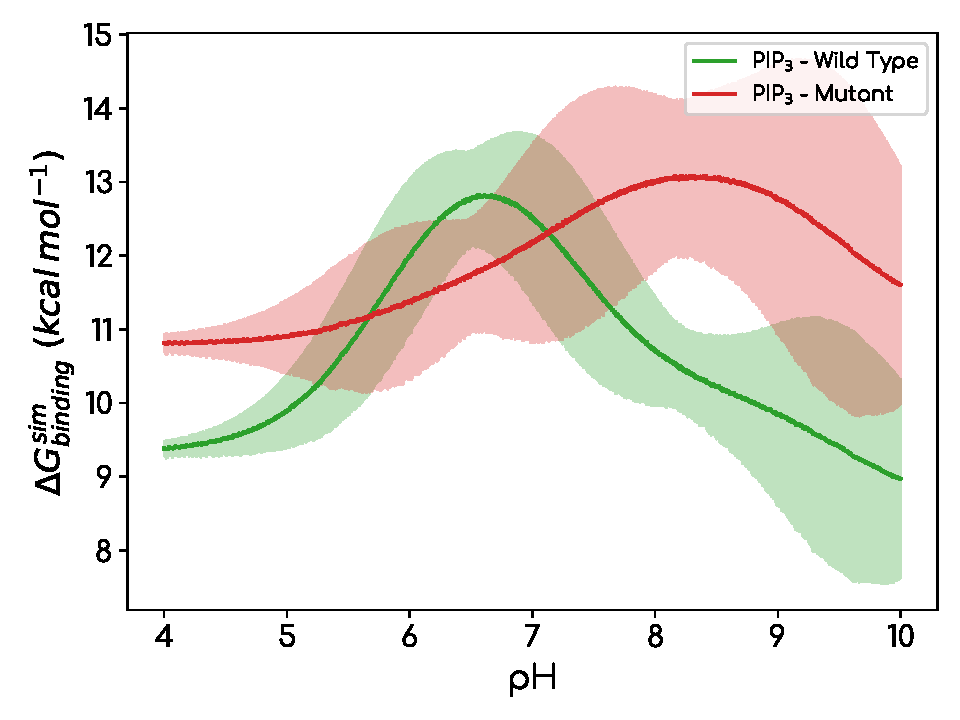
\includegraphics[width=0.45\linewidth]{figs/pip3_mutant_wild_type_delg_ph.pdf}
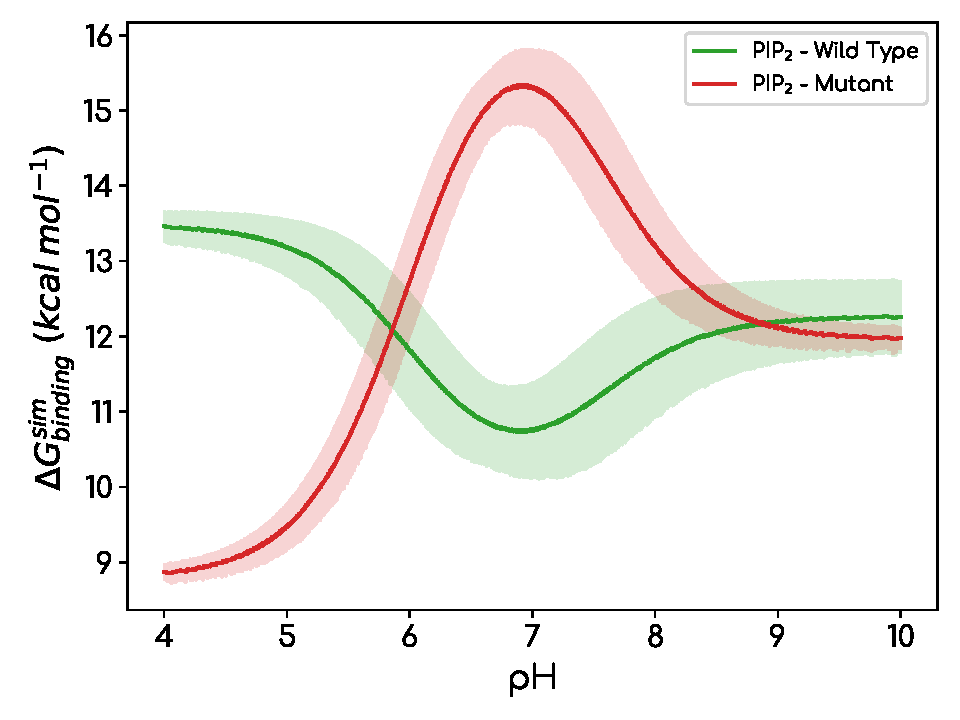
\includegraphics[width=0.45\linewidth]{figs/pip2_mutant_wild_type_delg_ph.pdf}
\caption{Free energy of binding as a function of pH for AKT1-WT(green) and AKT1-E17K mutant(red) in PIP$_3$(left) and PIP$_2$(right) systems respectively}
\label{figure2}
\end{center}
\end{figure}

       
\bibliographystyle{unsrt}
\bibliography{references}

\end{document}

